%\addbibresource{/home/jorgsk/phdproject/bibtex/jorgsk.bib}
\subsubsection{Transcriptome sequencing with RNA-seq}
The work presented in this thesis that deals with polyadenylation is based on
sequencing data from RNA (RNA-seq) made with the Illumina GAIIX platform. Se
http://www.ncbi.nlm.nih.gov/geo/query/acc.cgi?acc=GSE30567 for detailed
information about the data was generated.

RNA-seq is a technique used to obtain a quantitative measure of the relative
frequencies of the different species of RNA present in a sample. RNA-seq was
introduced in 2008 \cite{nagalakshmi_transcriptional_2008-1} and has been used
to compare the differential expression of genes, to discover new genes, and to
discover novel isoforms of known genes by finding new splice-sites and new 5\p
and 3\p terminals \cite{wang_rna-seq:_2009}.

Here we will go through the stages of the RNA-seq experiments that were
performed to produce the data that was analysed. We will then comment on the
stages of the experiment where biases can be introduced that affect the final
result. Finally we will discuss the matter of mapping the output of RNA-seq --
short RNA sequences called reads -- to the genome.

\subsubsection{RNA-seq and mapping: the method, errors, and biases}

\begin{itemize}
	\item The first step in an RNA-seq experiment is to isolate RNA from a cell
		sample obtained from a tissue or a cell culture

	\item Second, the RNA is divided into poly(A)+ and poly(A)- fractions. This
		is done by using a poly(T) primer that binds to the poly(A) tail of the
		mRNA. The RNA that binds the poly(T) primer is called the poly(A)+
		fraction and the RNA that does not bind the primer is separated and
		called the poly(A)- fraction.

	\item Next, the RNA samples are treated to remove ribosomal RNA. Since
		ribosomal RNA is by far the most abundant species of RNA in the cell,
		its removal will increase the sensitivity for detecting lowly expressed
		transcripts in the sample.

	\item Next, the single stranded RNA is converted into double stranded
		complementary DNA (cDNA). This is required because Illumina sequencers
		sequence DNA and not RNA. To turn RNA into cDNA it is necessary to use
		primers -- short sequences that bind RNA and DNA -- that the reverse
		transcriptase enzyme needs for synthesizing cDNA on the RNA template.
		At this step, it is important when studying polyadenylation that at
		least some of the primers are poly(T) primers, otherwise the poly(A)
		tail may not be converted into cDNA. Since the poly(T) primers can
		bind anywhere in the poly(A) tail, the lengths of the poly(A) tails
		will be reduced after this step.

	\item After this, the original single stranded RNA is degraded so only the
		double stranded cDNA remains.

	\item The next step is to fragment the cDNA into smaller pieces, usually by
		sound waves (sonication), to reach a desired average fragment size
		compatible with the sequencing machine (usually around 300 nt),

	\item Finally, short RNA adapters are added to the 3\p and 5\p ends of the
		cDNA and the cDNA is amplified from these adapters with PCR.  PCR
		amplification is necessary to get the volume of DNA required by the
		sequencing machines. Now the cDNA is ready for sequencing.

\end{itemize}

During sequencing, the double stranded cDNA is split into single strands, and
both strands are sequenced. This has the effect that sequencing outputs the
reverse-transcribed version of the original RNA molecule in addition to the
original. This is fortunate when studying polyadenylation, since the poly(A)
tail of a transcript is usually sequenced from the reverse-transcribed version
of the RNA (see Figure \ref{fig:polyT_seq}). That is, a polyadenylated 5\p
CCCGAAAA 3\p input will most often be output as 5\p TTTTCGGG 3\p from the
sequencing machine. This bias is due to the fact that sequencing happens in the
3\p to 5\p direction, and that the read length is shorter than the fragment
length (76 bp vs 300 bp in Figure \ref{fig:polyT_seq}).

It is important to note that when sequencing homopolymers (single-nucleotide
repeat sequences) like poly(A) or poly(T) stretches, there is a slight increase
in sequencing error rates with the Illumina platform
\cite{minoche_evaluation_2011}. This implies that when sequencing a poly(A)
sequence, other nucleotides than just A will be reported with a higher
probability compared to the rest of the output sequence.

\begin{figure}[htb]
	\begin{center}
		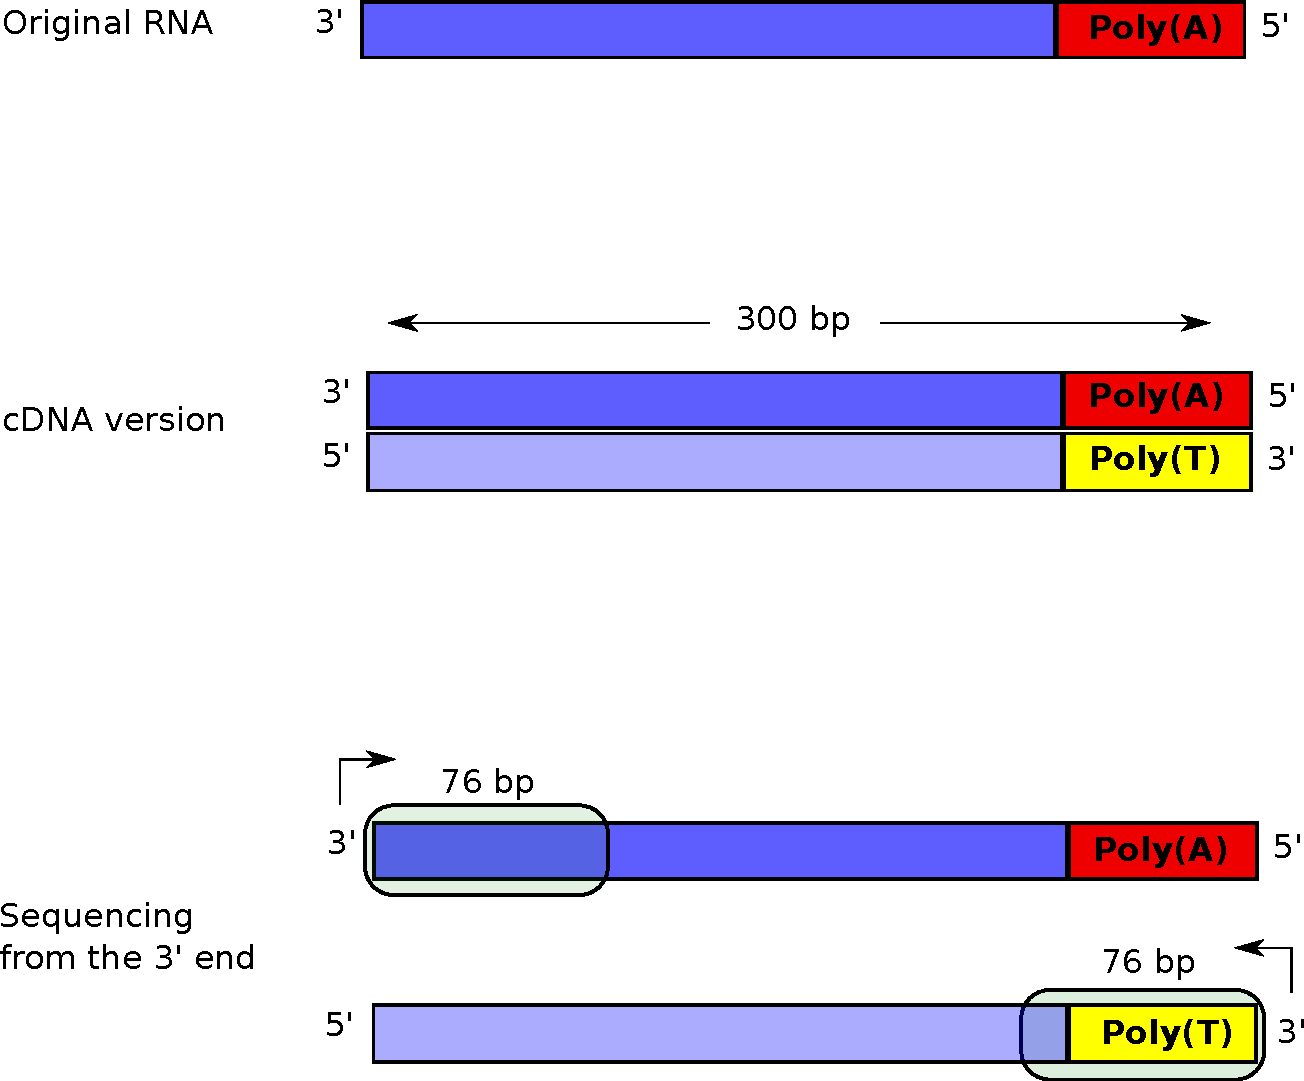
\includegraphics[scale=0.4]{figures/introduction/polyT_sequencing.pdf}
	\end{center}
	\caption{When sequencing poly(A) sites it is normally the
	reverse-transcribed version of the transcript that is actually sequenced}
	\label{fig:polyT_seq}
\end{figure}

\subsubsection{Mapping reads to the genome}
The sequence-snippets that are output from sequencing machines are called
reads, and generally come in sizes from 30 to 500 basepairs, depending on the
technology used. For the data used in this study, the read size was 76
basepairs.

If a reference genome exists for the organism from which the RNA sample was
taken, these reads can be mapped to that genome to find out where the RNA
originated from. Mapping a read to the genome means trying to find where the
RNA-snippet from the sequencing machine originated from. All methods used for
mapping allow for mismatches between the read and the genome to allow for
sequencing errors. 
